%\documentclass[tikz,border=3pt,convert={density=600,outext=.png}]{standalone}
\documentclass[tikz,border=3pt]{standalone}

\usepackage{tikz}
\usetikzlibrary{shapes,positioning,calc,arrows}

\begin{document}
	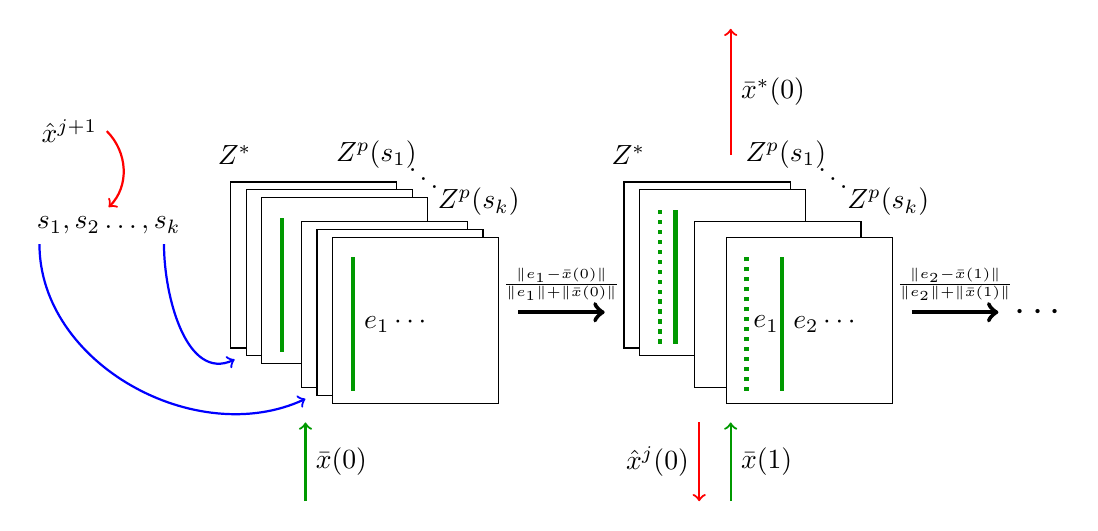
\begin{tikzpicture}
		\tikzstyle{z_matrix} = [draw, rectangle, minimum width = 60, minimum height = 60,fill=white];

			\node (meas_fun) at (0.7,0.5) {$s_1,s_2\dots,s_k$};	

			\node (control_vect) at ($(meas_fun)+(-0.5,1.2)$) {$\hat x^{j+1}$};
			\path[->,thick,red] (control_vect.east)  edge[out = -45, in = 45, right] (meas_fun.north); 

			\node[z_matrix] (z_1) at ($(meas_fun)+(2.6,-0.5)$) {};
			\node[z_matrix] at ($(z_1)+(0.2,-0.1)$) {};
			\node[z_matrix] at ($(z_1)+(0.4,-0.2)$) {};
			
			\node[z_matrix] at ($(z_1)+(0.9,-0.5)$) {};
			\node[z_matrix] at ($(z_1)+(1.1,-0.6)$) {};
			\node[z_matrix] at ($(z_1)+(1.3,-0.7)$) {};
			
			\path[->,thick,blue] ([xshift=20]meas_fun.south)  edge[out = -90, in = -155, right] ($(z_1)+(-1,-1.2)$);
			\path[->,thick,blue] ([xshift=-25]meas_fun.south)  edge[out = -90, in = -155, right] ($(z_1)+(-0.1,-1.7)$);
			
			\node at ($(z_1)+(-1,1.4)$) {$Z^*$};
			
			\node at ($(z_1)+(0.8,1.4)$) {$Z^p(s_1)$};
			\node at ($(z_1)+(1.4,1.2)$) {$\ddots$};
			\node at ($(z_1)+(2.1,0.8)$) {$Z^p(s_k)$};

			\draw[ultra thick, green!60!black] ($(z_1)+(-0.4,-1.1)$) -- ($(z_1)+(-0.4,0.6)$);
			\draw[ultra thick, green!60!black] ($(z_1)+(0.5,-1.6)$) -- node[right,black] {$e_1\cdots$} ($(z_1)+(0.5,0.1)$);
			
			\draw[->, thick, green!60!black] ($(z_1)+(-0.1,-3)$) -- node[right,black] {$\bar x(0)$} ($(z_1)+(-0.1,-2)$);

			\node[z_matrix] (z_2) at ($(z_1)+(5,0)$) {};
			\node[z_matrix] at ($(z_2)+(0.2,-0.1)$) {};
			
			\node[z_matrix] at ($(z_2)+(0.9,-0.5)$) {};
			\node[z_matrix] at ($(z_2)+(1.3,-0.7)$) {};
			
			\node at ($(z_2)+(-1,1.4)$) {$Z^*$};
			\node at ($(z_2)+(1,1.4)$) {$Z^p(s_1)$};
			\node at ($(z_2)+(1.6,1.2)$) {$\ddots$};
			\node at ($(z_2)+(2.3,0.8)$) {$Z^p(s_k)$};
			
			\draw[->, ultra thick] ($(z_1)+(2.6,-0.6)$) -- node [above] {\scriptsize$\frac{\| e_1-\bar x(0)\|}{\|e_1\|+\|\bar x(0)\|}$} ($(z_1)+(3.7,-0.6)$);
			
			\draw[ultra thick, dotted, green!60!black] ($(z_2)+(-0.6,-1)$) -- ($(z_2)+(-0.6,0.7)$);
			\draw[ultra thick, dotted, green!60!black] ($(z_2)+(0.5,-1.6)$) -- ($(z_2)+(0.5,0.1)$);

			\draw[->, thick, red] ($(z_2)+(0.3,1.4)$) -- node[right,black] {$\bar x^*(0)$} ($(z_2)+(0.3,3)$);

			\draw[<-, thick, red] ($(z_2)+(-0.1,-3)$) -- node[left,black] {$\hat x^j(0)$} ($(z_2)+(-0.1,-2)$);
				
			\draw[ultra thick, green!60!black] ($(z_2)+(-0.4,-1)$) -- ($(z_2)+(-0.4,0.7)$);
			\node at ($(z_2)+(0.75,-0.75)$) {$e_1$};
			\draw[ultra thick, green!60!black] ($(z_2)+(0.95,-1.6)$) -- node[right,black] {$e_2\cdots$} ($(z_2)+(0.95,0.1)$);	

			\draw[->, thick, green!60!black] ($(z_2)+(0.3,-3)$) -- node[right,black] {$\bar x(1)$} ($(z_2)+(0.3,-2)$);
			
			\draw[->, ultra thick] ($(z_2)+(2.6,-0.6)$) -- node [above] {\scriptsize$\frac{\|e_2-\bar x(1)\|}{\|e_2\|+\|\bar x(1)\|}$} ($(z_2)+(3.7,-0.6)$);
			\node at ($(z_2)+(4.2,-0.6)$) {\Large $\cdots$};
	\end{tikzpicture}
\end{document}